\documentclass[../main.tex]{subfiles}
\graphicspath{{\subfix{../IMAGES/}}}

\begin{document}
\localtableofcontents

\subsection{Introduction}
The available hydraulic power is given by : $P_h = \rho Q E (W)$ and the machine power output P(W) gives a turbine efficiency of $\eta^T = \frac{P}{P_h}$.\\

\begin{figure}[hbt!]
    \centering
    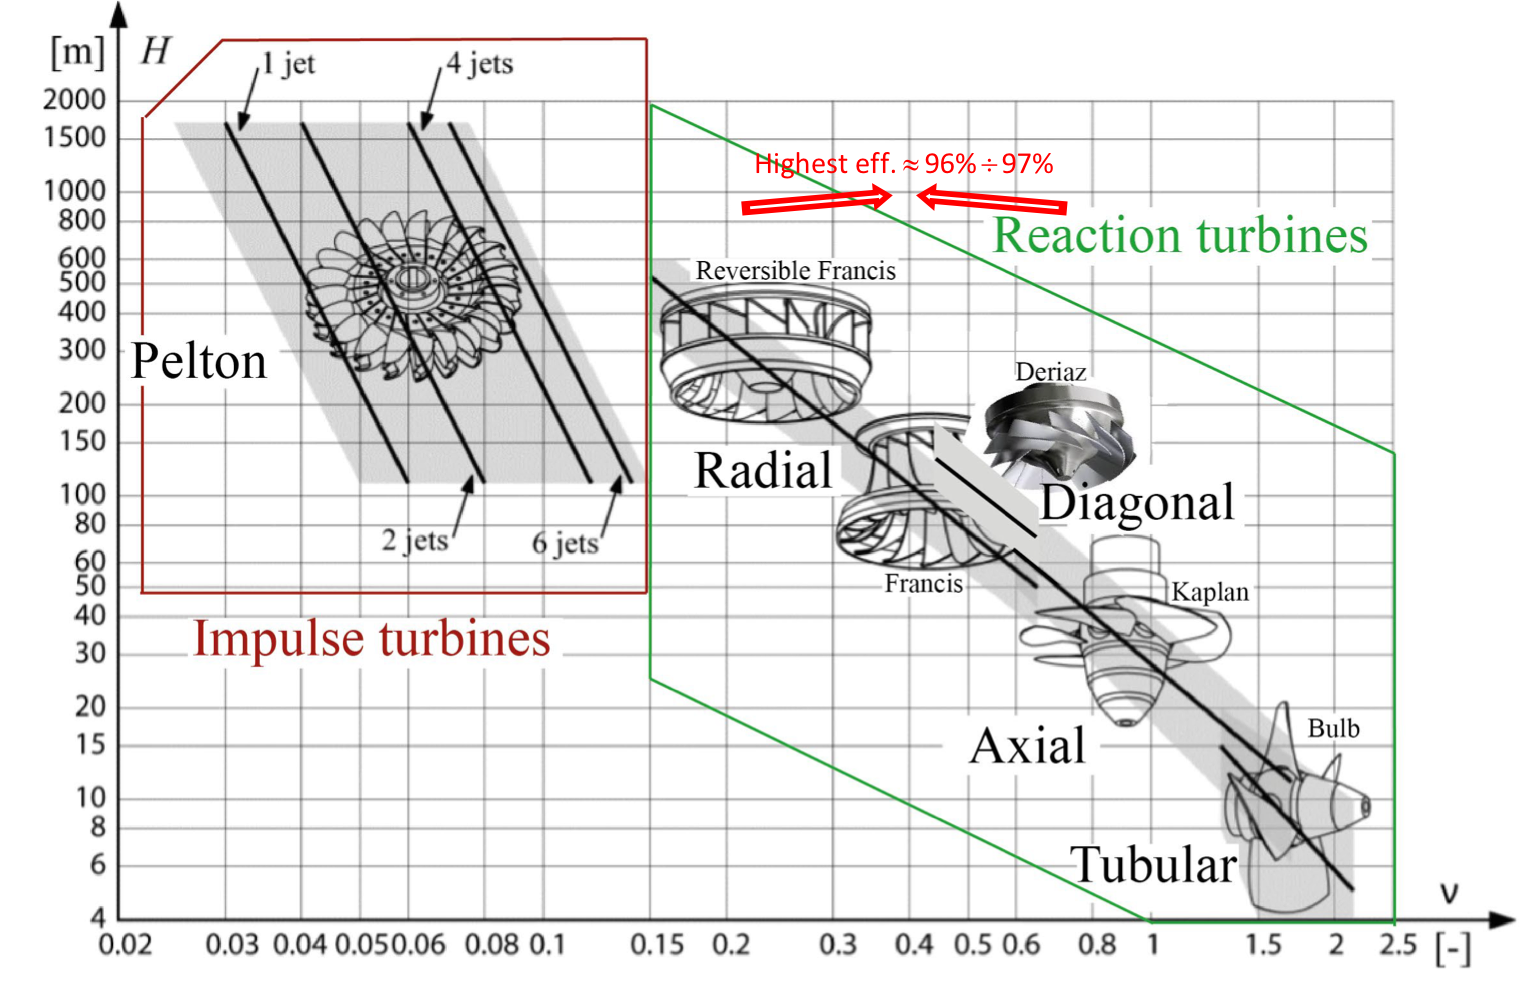
\includegraphics[width=0.8\linewidth]{IMAGES/Hydraulic/Hydrau1.png}
\end{figure}
With \begin{equation}
    v = 2^{1/4} \pi^{1/2} n \frac{Q^{1/2}}{E^{3/4}}
\end{equation}
\begin{itemize}
    \item Q the discharge $(m^3 s^{-1})$\\
    \item n the speed $(s^{-1})$\\
\end{itemize}

There exists multiple sorts of centrifugal pumps : \begin{table}[hbt!]
    \centering
    \begin{tabular}{c|c}
         Flow orientation & Number of stages \\ \hline
        Radial & Single stage\\
        Mixed-flow & two stages\\
        Axial & multistage\\
    \end{tabular}
\end{table}
Pumps for storage applications are mainly of the radial-flow type.

The local mean flow specific energy is given by : \begin{equation}
    h_t = \frac{p}{\rho} + gZ + \frac{C^2}{2} + Cste
\end{equation}

Which gives the available specific energy : \begin{equation}
    E = gH = gH_i - gH_{\overline{i}} = g(Z_B - Z_{\overline{B}}) - \sum gH_r
\end{equation}
With H the head.\\

The hydraulic power is given by : \begin{equation}
    P_h = \rho Q \times E = \rho Q g(H_l - H_{\overline{l}})
\end{equation}

They can be classified by : \begin{table}[hbt!]
    \centering
    \begin{tabular}{p{.28\textwidth}|p{.28\textwidth}|p{.28\textwidth}}
        By types & By head & Power capacity \\ \hline
        Storage, pumped-storage, run of river, offshore & High (>300m), medium (30-300m), low (<30m) & Large (>100MW), medium (25-100MW), small (1-25MW), mini (100kW-1MW), micro (<100kW)
    \end{tabular}
\end{table}

If we consider steady flow and straight stream lines, the specific energy balance between two points in a pipe : $gH_1 = gH_2 + \sum_{1:2}(gH_r)_i$. The discharge balance indicates : $Q_1 = Q_2$  and the mass conservation equations gives us : $A_1C_1 = A_2C_2$\\

The pip distributed losses are given by : \begin{equation}
    gH_{r 1:2} = \lambda(Re; k/D_h) \frac{L_{\hat{12}}}{D_h} \frac{C^2}{2} (J kg^{-1})
\end{equation}
With \begin{itemize}
    \item $\lambda$ the local loss coefficient
    \item $Re$ the Reynolds number $Re = \frac{CD_h}{\nu}$ (we take $Re>10^6$) 
    \item $k$ the roughness
    \item $D_h$ the hydraulic diameter $D_h = \frac{4A}{P_{wet}}$
\end{itemize}


\begin{figure}[hbt!]
    \centering
    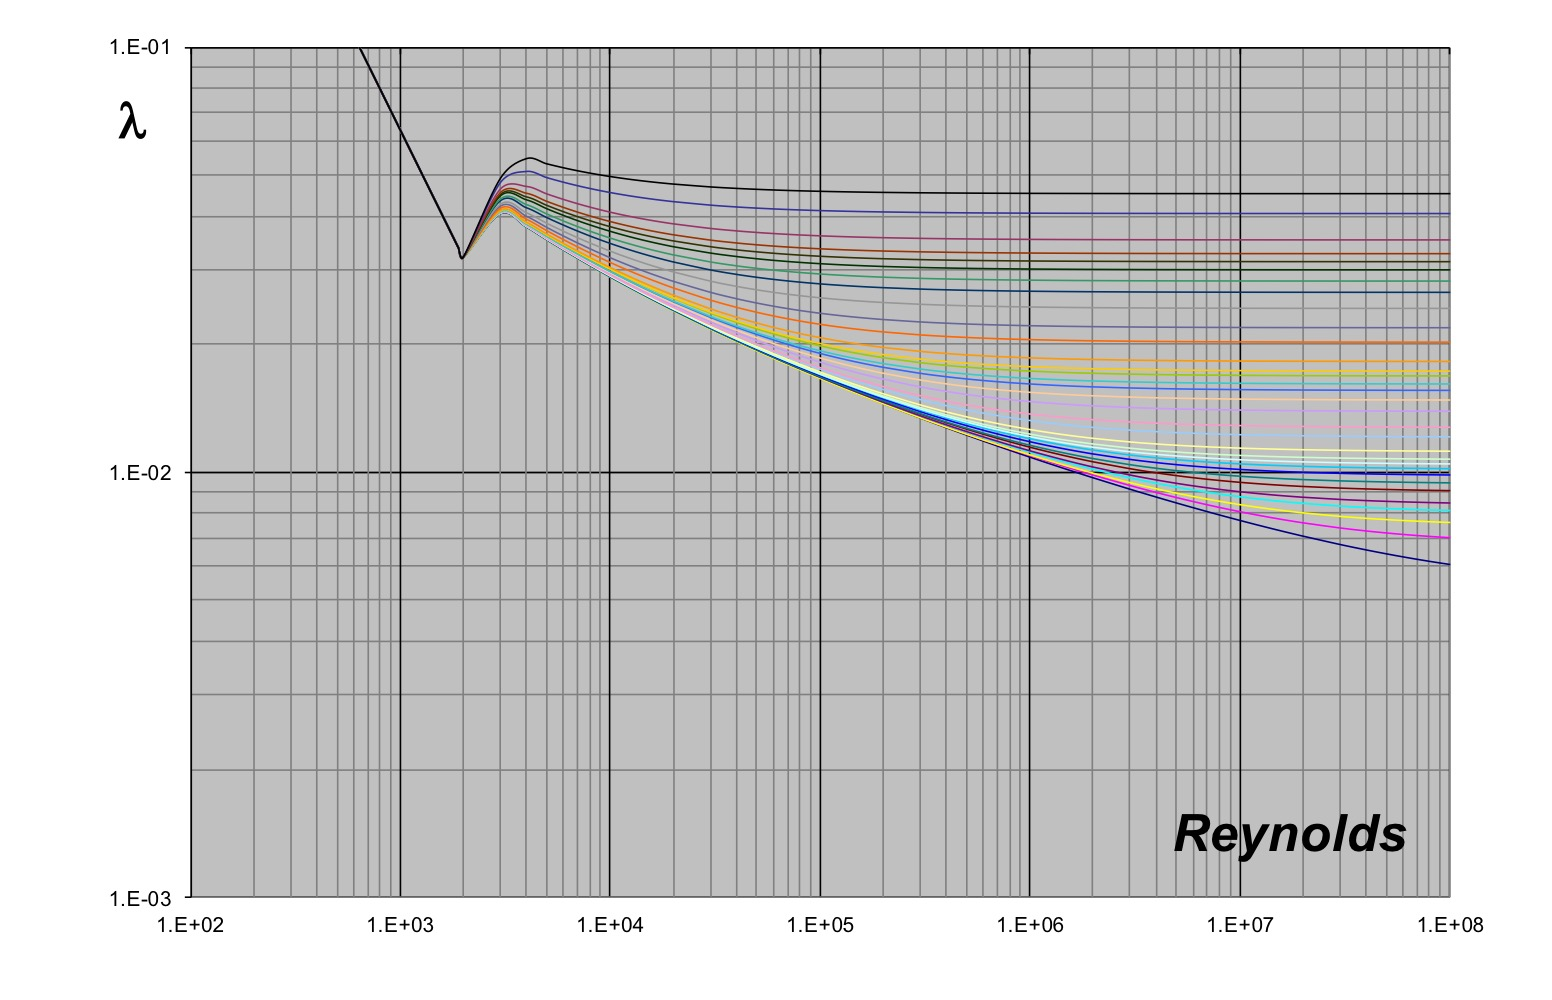
\includegraphics[width=0.8\linewidth]{IMAGES/Hydraulic/IMG_0178.jpeg}
\end{figure}

From the churchill empirical formula, we have \begin{equation}
    \begin{gathered}
        \lambda(Re; k_s/D) = 8 [(\frac{8}{Re})^{12} + \frac{1}{(A+B)^{3/2}}]^{1/12}\\
        A = [2.457 \ln \frac{1}{(7/Re)^{0.9} + 0.27 \frac{k_s}{D}}]^{16}\\
        B = [\frac{37530}{Re}]^{16}
    \end{gathered}
\end{equation}

There exists different kind of losses : \begin{itemize}
    \item Distributed losses $gH_{r 1:2} = \lambda(Re; k/D_h) \frac{16}{\pi^2} \frac{L}{D_h^5} \frac{Q^2}{2}$
    \item Singular losses for the ith component $gH_{ri} = K_i \frac{1}{A_i^2} \frac{Q^2}{2}$
    \item General formula $gH_{r x:y} = \sum_{i=1}^n K_i \frac{A_{ref}^2}{A_i^2} \frac{Q^2}{2A_{ref}^2}$
\end{itemize}

It can be summarized in $gH_{r 1:2} = (1-\frac{A_1}{A_2})^2 \frac{C_1^2}{2} = K \frac{C_2^2}{2}$\\

\quad \underline{Rotating train dynamics :}\\
\begin{equation}
    J \frac{d\omega}{dt} = T + T_{el}
\end{equation}
With \begin{itemize}
    \item J the inertia
    \item $\omega$ the angular speed
    \item in case of synchronous conditions $T = -T_{el}$
    \item in case of load rejection $T_{el} = 0 \Rightarrow \frac{d\omega}{dt} = T>0$
    \item the grid frequency is either $f_{grid} = 16 \frac{2}{3}, 50, 60 Hz$
    \item the rotating frequency is then $n = \frac{2 f_{grid}}{z_p} (Hz)$, $z_p$ the number of poles
\end{itemize}

In pumping mode, we have \begin{equation}
    gH_l - gH_{\overline{l}} = g(Z_B - Z_{\overline{B}}) + \sum gH_r
\end{equation}

\quad \underline{Power exchange :}\\
\begin{itemize}
    \item Hydraulic power $P_h = P_l - P_{\overline{l}} (W)$
    \item Work-generating (turbine) $P = \eta^T P_h >0$
    \item Work-absorbing (pump) $P_h = \eta^P P <0$
\end{itemize}

\quad \underline{Turbine mechanical power :}\\
\begin{equation}
\begin{gathered}
    P_m = P + P_{lm}\\
    P_t = P_m + P_{rm}\\
    P_h = P_t + \sum P_r + \sum P_q\\
    \end{gathered}
\end{equation}
With \begin{itemize}
    \item $P$ the machine power
    \item $P_{lm}$ the external power losses
    \item $P_m$ the runner mechanical power
    \item $P_{rm}$ the internal mechanical power losses
    \item $P_t$ the extracted power
    \item $P_r$ the flow power dissipation
    \item $P_q$ the leakage flow power
\end{itemize}
The extracted energy is given by $E_t = \frac{P_t}{\rho Q_t}$ and the driving torque by $P_t = \omega T_t$.\\

\quad \underline{Pump mechanical power :}\\
\begin{equation}
\begin{gathered}
    P = P_m + P_{lm}\\
    P_m = P_t + P_{rm}\\
    P_t = P_h + \sum P_r + \sum P_q\\
    \end{gathered}
\end{equation}

\subsection{Classification of Hydraulic runners}
\begin{figure}[hbt!]
    \centering
    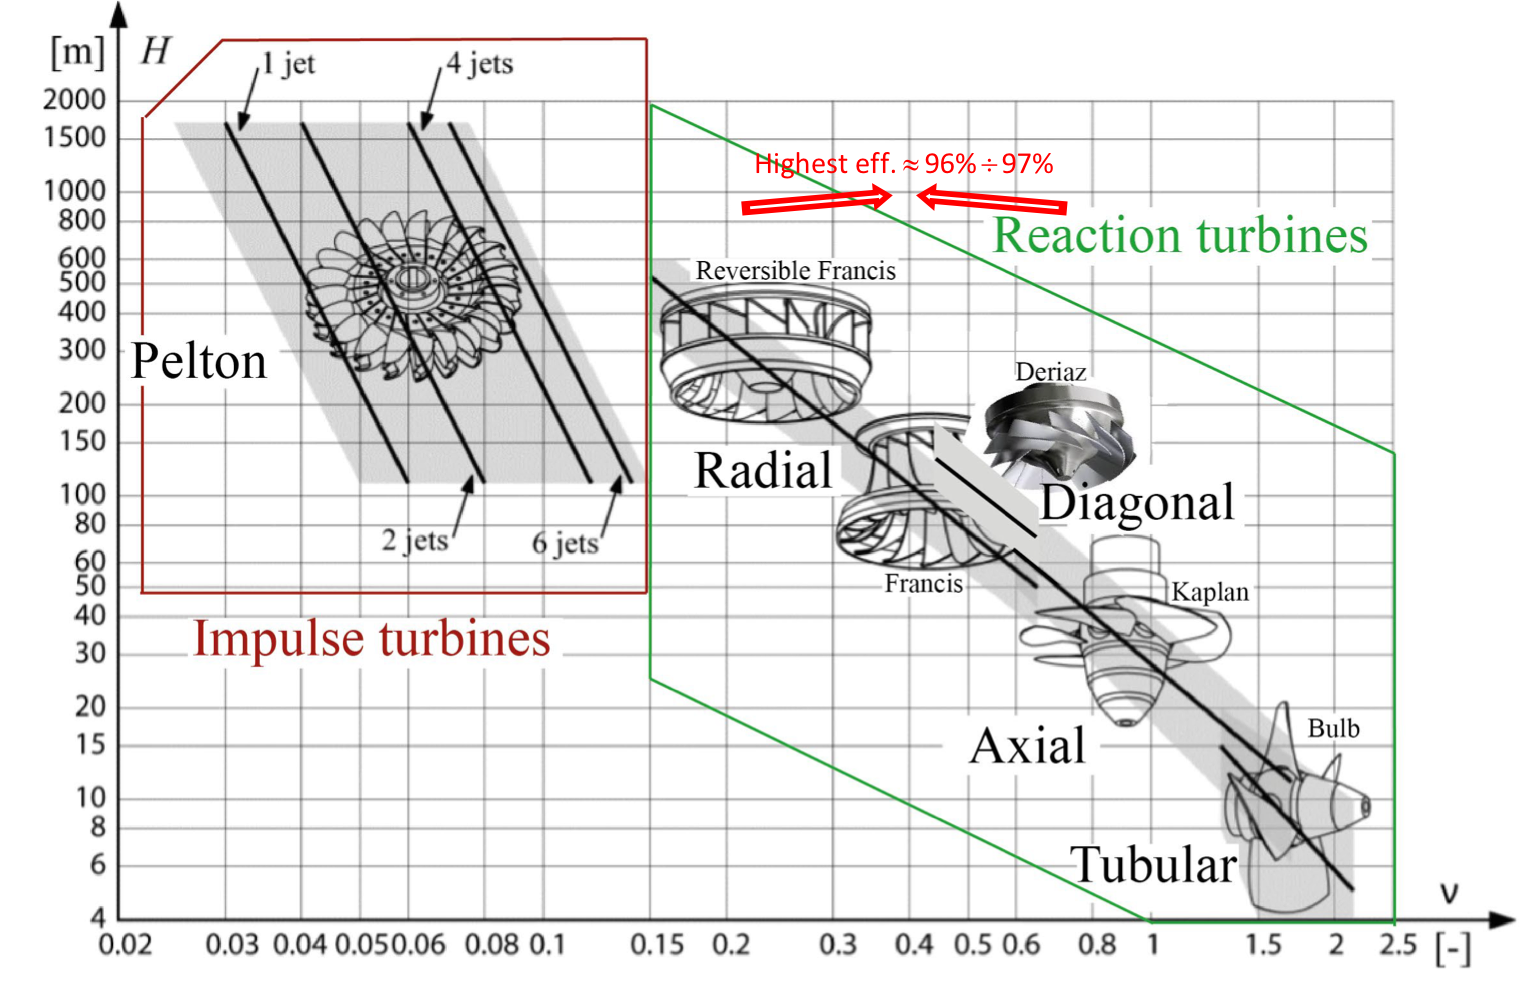
\includegraphics[width=0.8\linewidth]{IMAGES/Hydraulic/Hydrau1.png}
\end{figure}

With $H$ the head in m, $Q$ the discharge in $m^3 s^{-1}$ and $N$ the speed in min${}^{-1}$.\begin{equation}
    \nu = 2^{1/4} \pi^{1/2} n \frac{Q^{1/2}}{E^{3/4}}
\end{equation}
This is a dimensionless angular speed condition. \\
We can also define : \begin{itemize}
    \item Discharge coefficient $\varphi = \frac{C_m}{U}$ ($C_m = \frac{Q}{A}$ : meridional velocity, $U = \omega R$ : tangential velocity)
    \item Specific energy coefficient $\psi = \frac{E}{U^2/2}$
    \item Specific speed $\nu = \frac{\varphi^{1/2}}{\psi^{3/4}} = \frac{\omega}{\pi^{1/2} 2^{3/4}} \frac{\lvert Q \rvert^{1/2}}{E^{3/4}}$
\end{itemize}

\subsection{Hydraulic energy conversion}
The acceleration of the flow can be written as $\frac{DC}{Dt} = \frac{\partial C}{\partial t} + (C\cdot \nabla) C = \frac{\partial C}{\partial t} + \nabla \frac{C^2}{2}- C\times \Omega$.\\

The incompressible flow equation is $\frac{1}{\rho} \frac{D\rho}{Dt} = -\nabla C = 0$\\

For viscous and turbulent flow, we have $\frac{DC}{Dt} = -\nabla (\frac{p}{\rho} + gZ) + \nabla (2\nu D + \frac{\tau_t}{\rho})$\\

In an elbow, we have the specific energy balance : $\frac{d}{dn}(\frac{p}{\rho} + gZ) = -\frac{C^2}{R} + \nabla (2\nu D + \frac{\tau_t}{\rho})$
As the local balance along a streamline between two points : $h_1 = h_2 - \int_{12} [\nabla \cdot (2\nu D + \frac{\tau_t}{\rho})] dL + \int_{12} \frac{\partial C}{\partial t} dL$\\

For a pipe, the flow power balance and flow power dissipation are : \begin{equation}
    \begin{gathered}
        \int_{A_1 \cup A_2} \rho h_t C\cdot n dA = -\int_V \frac{\partial }{\partial t}(\frac{C^2}{2})\rho dV \text{(0 if stationnary)} + \int_(\rho (2\nu D + \frac{\tau_t}{\rho})\cdot C)\cdot n dA \text{(0 is homogeneous)} - \int_V (\Phi + \Pi) \rho dV\\
        P_{r, 1:2} = -\int_V (2\nu D + \frac{\tau_t}{\rho}D)\rho dV = -\int_V (\Phi + \Pi) \rho dV, \Phi \text{ the viscosity }, \Pi \text{ the turbulence}\\
    \end{gathered}
\end{equation}

The flow weighted average of local specific total energy is $gH = \frac{P_h}{\rho Q} = \pm \int_A (\frac{p}{\rho} + gZ + \frac{C^2}{2}) \frac{C\cdot n dA}{Q}\geq 0$.\\

The discharge can be expressed as $Q = \int_A C \cdot ndA (m^3 s^{-1}$ and the flow power $P_h = \int_A (\frac{p}{\rho} + gZ + \frac{C^2}{2}) \rho C\cdot n dA (W)$

\begin{itemize}
    \item Hydraulic power $P_h = \rho Q E$
    \item Power lost in spiral case $P_{rsc} = \rho Q E_{rsc}$
    \item Power lost in stay vanes $P_{rv} = \rho Q E_{rv}$
    \item Power lost in guide vanes $P_{ro} = \rho Q E_{ro}$
    \item Transferred Power $P_t = \rho Q_t E_t$
    \item Power lost in the blades $P_{rb} = \rho Q_t E_{rb}$
    \item Power lost through leakage $P_{rq} = \rho q_r (E_t+ E_{rb})$
    \item Power lost in the draft tube $P_{rb} = \rho Q E_{rd}$
    \item $E = E_{rsc} + E_{rv} + E_{ro} + E_t + E_{rb} + E_{rd}$
\end{itemize}

\underline{Labyrinth seal leakage :}\\
$gH_{rSeal} = K_{vSeal} \frac{C^2}{2}$, $K_{vSeal} = z_{step} + \lambda(Re, \frac{k_s}{D_{hSeal}}) \frac{\sum L_{seal}}{D_{hseal}}$\\
We have the equivalent diameters : \begin{itemize}
    \item $A_{seal}= (2+ \frac{\delta R}{R_{seal}}) \pi R_{seal} \delta R$
    \item $P_{seal} = (2+\frac{\delta R}{R_{seal}})2\pi R_{seal}$
    \item $D_{hSeal} = 2\delta R$
\end{itemize}

For a turbine, we have $E = E_t + \sum E_r^T$, $\eta_e^T = \frac{E_T}{E}$ and $Q = Q_t + Q_r$, $\eta_q^T = \frac{Q_t}{Q}$ whereas for a pump $E_t = E + \sum E_r^P$, $\eta_e^P = \frac{E}{E_t}$ and $Q_t = Q+Q_r$, $\eta_q^P = \frac{Q}{Q_t}$\\

\begin{figure}[hbt!]
    \centering
    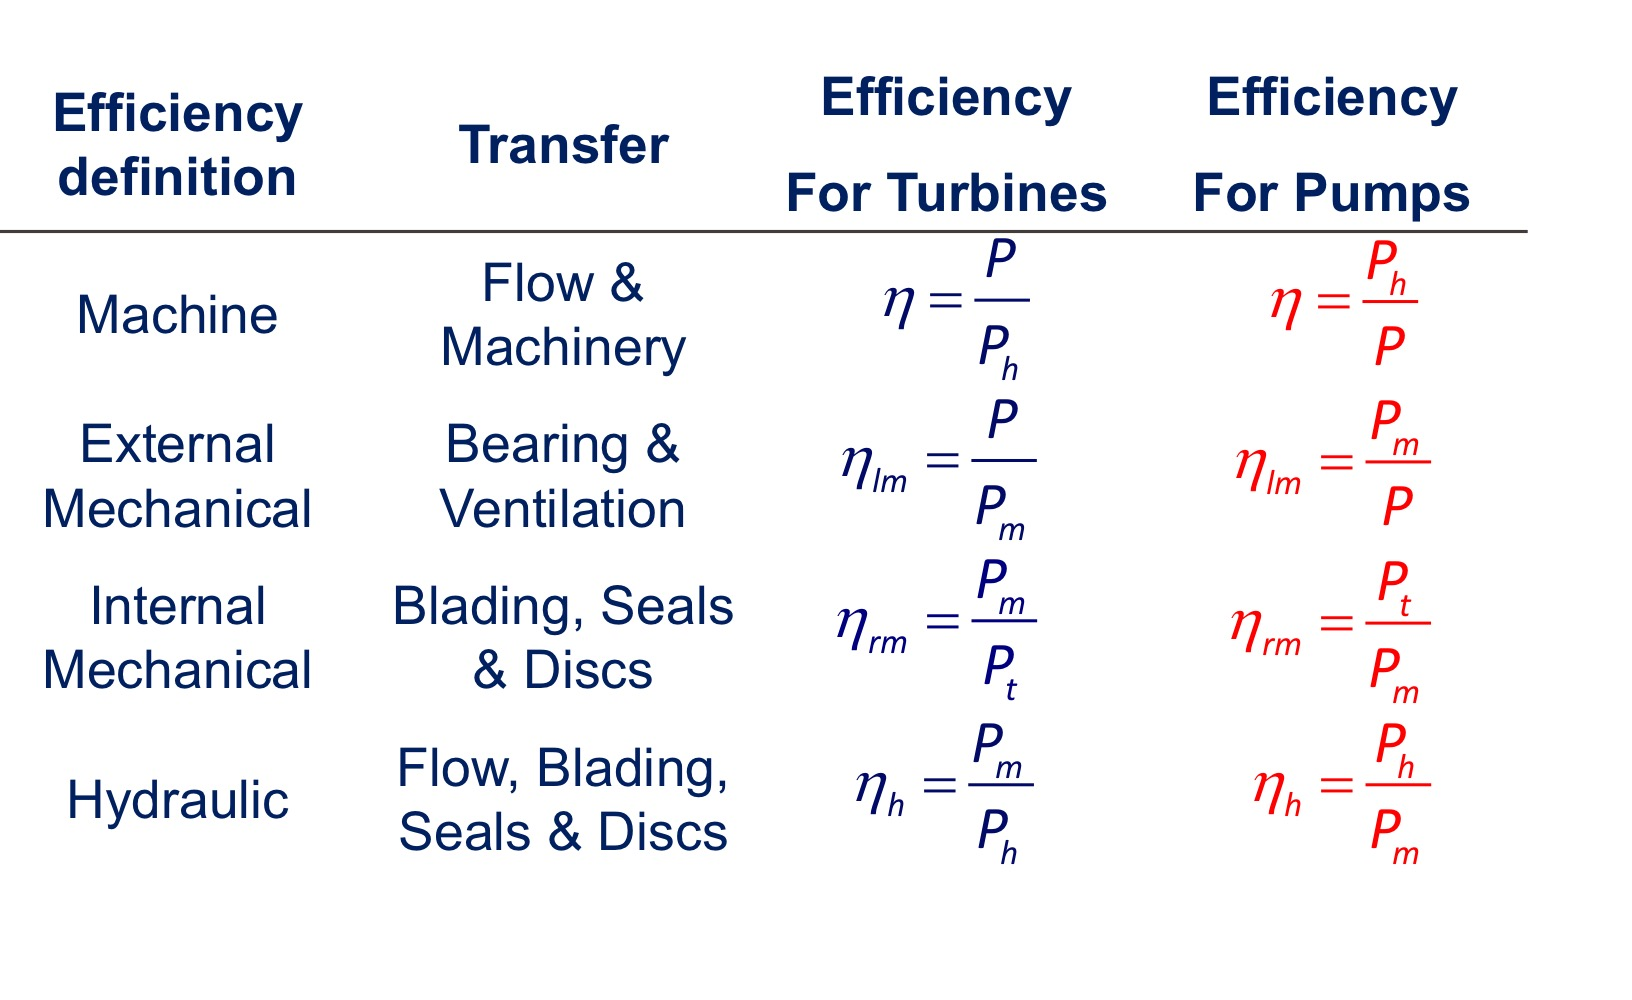
\includegraphics[width=0.6\linewidth]{IMAGES/Hydraulic/IMG_0182.jpeg}
\end{figure}

With $z_{units}$ the number of units and $Q_{instal}$ the installation discharge, we have the targeted unit specific head : $\nu = \frac{\omega}{\pi^{1/2} 2^{3/4}} \frac{(Q_{inst}/z_{units})^{1/2}}{E^{3/4}}$. \\
\warning We need to check for apparent power per poles : Air cooling < $28MVA$ < Water cooling < $35 MVA$\\

\subsubsection{Turbines characteristic curves}
\begin{itemize}
    \item IEC discharge factor : $Q_{nD} = \frac{Q}{nE^{3}} = \frac{Q_{ED}}{n_{ED}}$
    \item IEC speed factor : $n_{QE} = \frac{nQ^{1/2}}{E^{3/4}} = n_{ED} \sqrt{Q_{ED}}$
\end{itemize}


\begin{figure}[hbt!]
    \centering
    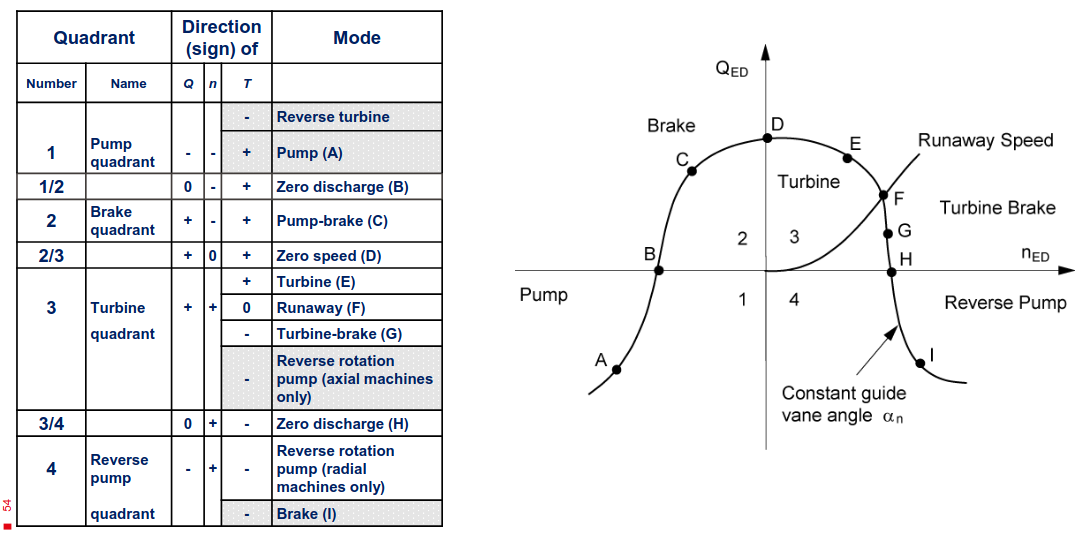
\includegraphics[width=0.8\linewidth]{IMAGES/Hydraulic/Screenshot from 2024-09-28 13-13-11.png}
\end{figure}

\subsection{Velocity triangle}

Because we are in a rotating frame, we have $\Vec{C} = \vec{U}+ \vec{W}$ with $\vec{C}$ the absolute flow velocity, the rotating velocity $\vec{U} = \vec{\omega} \times \vec{X} = \omega R$ and the relative flow velocity $\vec{W}$.\\

On a blade to blade view (view of the blade channel projected on the 2D plane on a iso-span line), we can define : \begin{itemize}
    \item Meridional component : $Cm = \frac{Q_t}{A}$
    \item Tangential component : $Cu = \frac{Cm}{\tan \alpha} = U- \frac{Cm}{\tan \beta}$ with $\alpha$ the absolute flow angle (guide vanes) and $\beta$ the relative flow angle (blade angle, hypotheses)
\end{itemize}

The trailing edge is the edge at the exit of the runner whereas the leading edge is the inlet section of the runner.

\begin{figure}[hbt!]
    \centering
    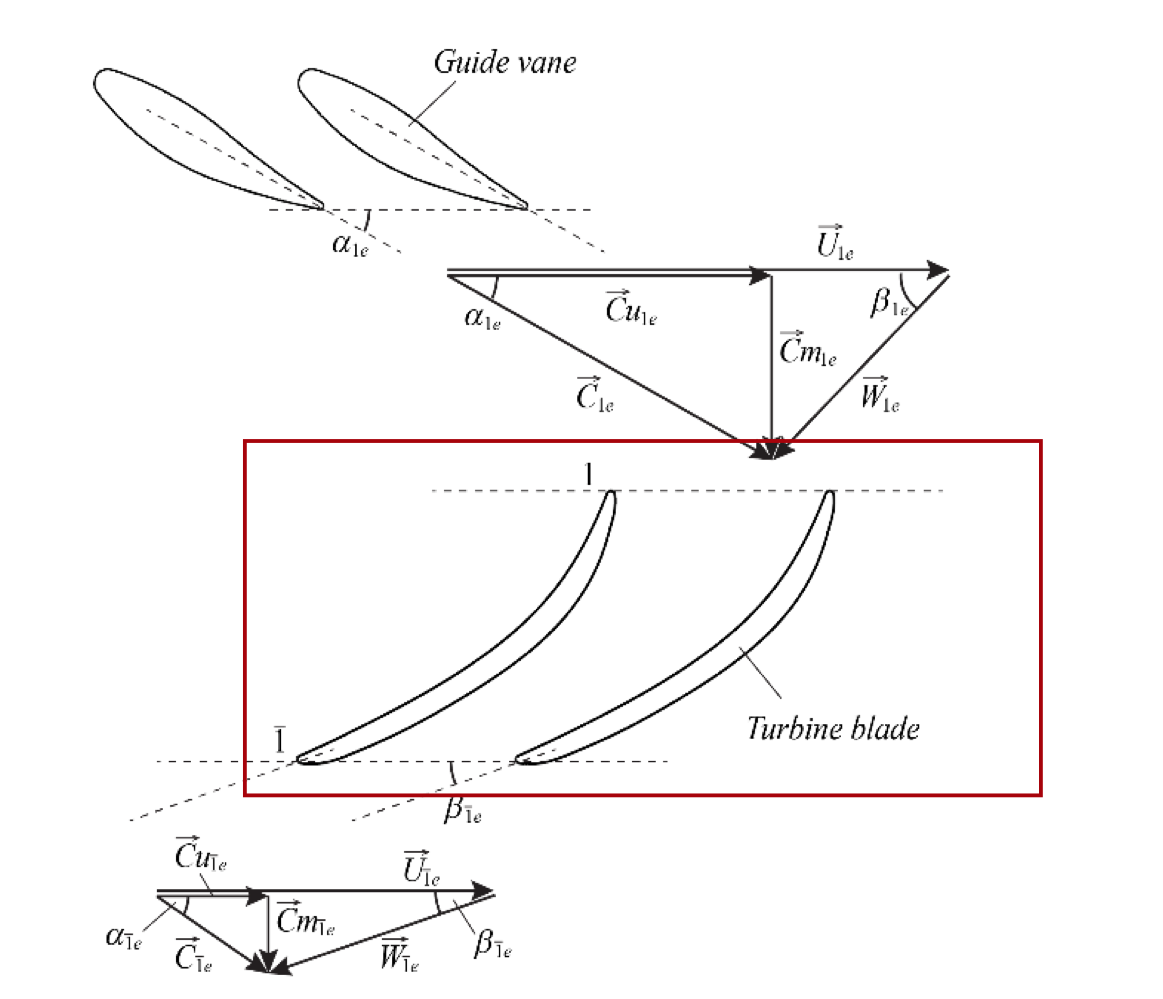
\includegraphics[width=0.8\linewidth]{IMAGES/Hydraulic/PNG image.png}
\end{figure}

Another view is the Meridional view : view of the blade projected on the 2D plane. Cut view following the curvature of the blade.

\quad \underline{Specific total rothalpy :}\\
\begin{itemize}
    \item Local rotational stagnation enthalpy : $h^{rel} = \frac{p}{\rho} + gZ - \frac{U^2}{2} + \frac{W^2}{2}+cste$
    \item Along a relative flow stream line : $h_1^{rel} = h_2^{rel} - \int_{12} [\nabla \cdot (2 \nu D + \frac{\tau_t}{\rho}) ]dL + \int_{12} \frac{\partial W}{\partial t}dL$
\end{itemize}

The relative acceleration is given by : $\frac{DC}{Dt} = \frac{DW}{Dt}\rvert_{relative frame} - 2\omega \times W + \omega \times (\omega \times X)$ with $\omega \times (\omega \times X) = \nabla (-\frac{U^2}{2})$. Then : \begin{equation}
    \frac{DW}{Dt} = [-\nabla (\frac{p}{\rho} + gZ - \frac{U^2}{2})] + (2\omega \times W) + \nabla \cdot (2\nu D + \frac{\tau_t}{\rho})
\end{equation}

We then have : \begin{itemize}
    \item the extracted specific energy : $E_t = C_1 U_1 - C_{\overline{1}} U_{\overline{1}} = U_1 Cu_1 - U_{\overline{1}} Cu_{\overline{1}}$ (Euler equation)
    \item the extracted power : $P_t = \int_{A_1 \cup A_{\overline{1}}} (-\frac{U^2}{2} + \frac{W^2}{2} - \frac{C^2}{2}) \rho C\cdot n dA = -\int (C\cdot U) \rho C\cdot n dA$
    \item resulting torque : $T_t = \frac{\rho Q_t E_t}{\omega} = \rho Q_t \frac{U_1 Cu_1 - U_{\overline{1}} Cu_{\overline{1}}}{\omega} = \rho Q_t (R_1 Cu_1 1 R_{\overline{1}} Cu_{\overline{1}})$
\end{itemize}

The global Euler equation is written as $E_t = k_{C_{u1e}} C_{1e} U_{1e} - k_{C_{u\overline{1}e}} C_{\overline{1}e} U_{\overline{1}e}$ with $k_{C_{ux}} = \lvert \frac{\int_{A_x} (C\cdot U) C \cdot n dA}{Q_t (C_x \cdot U_x)}\rvert$ in case of uniform flow at turbine inlet, we have $k = 1$. The index e informs that we are using the most external streamline possible; the streamline furthest away from the axis. If we compute it at the streamline on the mid-span, coefficients are equal to 1 for Pelton turbines. Otherwise, we have $k_{Cu1e} = 1$, $k_{Cu\overline{1e}} = \frac{1}{2}$. A reference case where at the inlet, both distributions of tangential and meridional components of the flow velocity are uniform and at the outlet the distribution of meridional component of flow velocity is uniform and the tangential component is of a solid body rotation of flow. This yields : $k_{Cu1e} = k_{Cm1e} = 1$ and $k_{Cu\overline{1e}} = \frac{1}{2}$, $k_{Cm\overline{1e}} = 1$.\\

It can be rewritten as $E_t = -k_{u\overline{1}e} U_{\overline{1}e}^2 + [\frac{R_{1e} A_{\overline{1}}}{R_{\overline{1}e} A_1} \frac{1}{\tan \alpha_{1e}} + k_{u \overline{1}e} \frac{1}{\tan \beta_{e\overline{1}}}] \frac{U_{\overline{1}e} Q_t}{A_{\overline{1}}} $.\\

The best efficiency is obtained when the outlet flow is only axial (for reaction machines): $Cu_{e\overline{1}} = 0$ to get $E_t = U_{1e} Cu_{1e}$\\

\quad \underline{Pump impeller :}\\
Assume swirl free inlet flow (axial flow).\\

The transferred power is then : $P_t = \rho Q_t U_{1e} [k_{u1e} U_{1e} - k_{u1e} \frac{1}{\tan \beta_{1e}} \frac{Q_t}{A_1}]$;\\


\subsection{Pelton turbines}
There exists horizontal and vertical shaft machines. Horizontal shaft allows a maximum of 2 nozzles. Vertical shaft allows up to 6 nozzles as more will generate too much turbulence in the inlet flow. \\
Pelton have an efficiency always around $95\%$ and does not change much with the flow output.\\

We have $C_1$ the jet velocity, $U_1$ the bucket velocity and $W_1$ the discharge flow velocity. The force acting on the bucket is then $F = 2\rho Q (C_1-U_1)$. The power extracted is then $P = FU_1 = 2\rho Q (C_1- U_1) C_1$\\

\warning At maximum power conditions, the rotating speed is half of the jet speed.\\
\begin{table}[hbt!]
    \centering
    \begin{tabular}{|c|c|c|}
        \hline
        Operation & Power & Force \\
        \hline
        Stopped & 0 & Max\\
        \hline

        Normal & Max & 0.5 Max\\
        \hline
        Runaway & 0 & 0\\ \hline
    \end{tabular}
\end{table}

Let $D_1$ be the pitch diameter, $d_0$ the jet diameter and $B_2$ the inner bucket width.\\

The speed factor can be described as $k_{u_1} = \frac{nD_1 \pi}{\sqrt{2gH}}$(similar to $n_{ED}$) and the normalized bucket load $\varphi_{B_2} = \frac{Q/z_0}{B_2^2 \pi/4 \sqrt{2gH}}$ (similar to $Q_{ED}$) with $z_0$ the number of jets.\\
Specific speed is defined by : $n_{ED} \sqrt{Q_{ED}} \propto \frac{D_1}{B_2}$.\\
To be feasible, we need $\frac{D_1}{B_2}>2.7$ and as large as we can to increase the efficiency of the machine.\\
If we have multiple units using the same penstock for two units, the efficiency of one unit when the other is out of operation, then $\eta_{3 \text{in operation}} = \eta_{2 \text{out of operation} } + 0.5\%$.\\
We can add inserts to control the flow and eliminate cavitation around the nozzle.\\

In the bucket, there is a periodic flow, simultaneous operation of many buckets, a stochastic characteristic of the flow.\\
Cavitation can appear on the buckets called : droplet cavitation; droplets of water with high velocity can change into steam when hitting the buckets.

\quad \underline{Model to prototype :}\\
We need to keep three variable constant : \begin{itemize}
    \item $Re = \frac{1}{\nu} B_2 \sqrt{H} $ : geometric
    \item $Fr = \frac{1}{\sqrt{g}} \sqrt{\frac{H}{B_2}}$ : cinematic
    \item $We = \sqrt{\frac{\rho}{\gamma}} \sqrt{H B_2}$ : dynamic
\end{itemize}
In practice, we can only respect the Froude number equality. Then : \begin{equation}
    \Delta \eta = \eta_{proto} - \eta_{model} = 5.7(1-C_{FR}^{0.3})(\frac{\varphi_{B2}}{\sqrt{\psi_1}})^2 + 1.95\cdot 10^{-6} (C_{We}-1) (\frac{\sqrt{\psi_1}}{B_2})^2 + 10^{-8} (C_{Re}-1) (\frac{\sqrt{\psi_1}}{B_2})^2
\end{equation}
With $C_{Re} = \frac{Re_p}{Re_m}$.
Buckets start to rupture after about $24000$ operation hours.\\

Water flow can damage the runners if it contains minerals. Buckets need to be coated to avoid erosion : hard coating.\\

\subsection{Reaction turbines}


There exists two kinds of spiral case : Double curvature (continuous, for high head) and Piguet type (notch around the stay vanes, less expensive, more suitable for small geometries).\\
Stay vanes are welded.\\
For low head turbines, we can have a semi spiral case; water comes from three channel on the same side of the runner. Because of the stress generated, impossible to use double curvature/piguet.\\
Guide vanes can move and change pitch. The minimum angle between two of them is $\theta_0 = \frac{2\pi}{z_0}$ with $z_0$ the number of GV.\\
The GV rotate around their center. The radius at their end is given by : $R_2 = R_0 \sqrt{ (\frac{l}{R_0} - \sin \alpha_0)^2 + \cos^2 \alpha_0}$ where $l$ is the distance from the center of rotation to the end of the GV, $\alpha_0$ is the angle between the center of rotation and the tangential of the circle and $\alpha_{20}$ the angle of the GV with respect to the tangential of the inner circle (at the end of the GV) : $\cos \alpha_{20} = \frac{R_0}{R_2} \cos \alpha_0$\\

\subsubsection{Francis runners}

The outlet angle $\sin\beta_{\overline{1}} = \frac{z_b B_{\overline{1}}}{2\pi R_{\overline{1}}}$ with $B_{\overline{1}}$ the distance between two blades.\\

Let $\beta_{b1e}$ the pitch angle at the leading edge and $\beta_{1e}$ the relative velocity angle. There might be a mismatch between them and we define the relative flow incidence : $i = \beta_{1e} - \beta_{b1e}$.\\

\begin{figure}[hbt!]
    \centering
    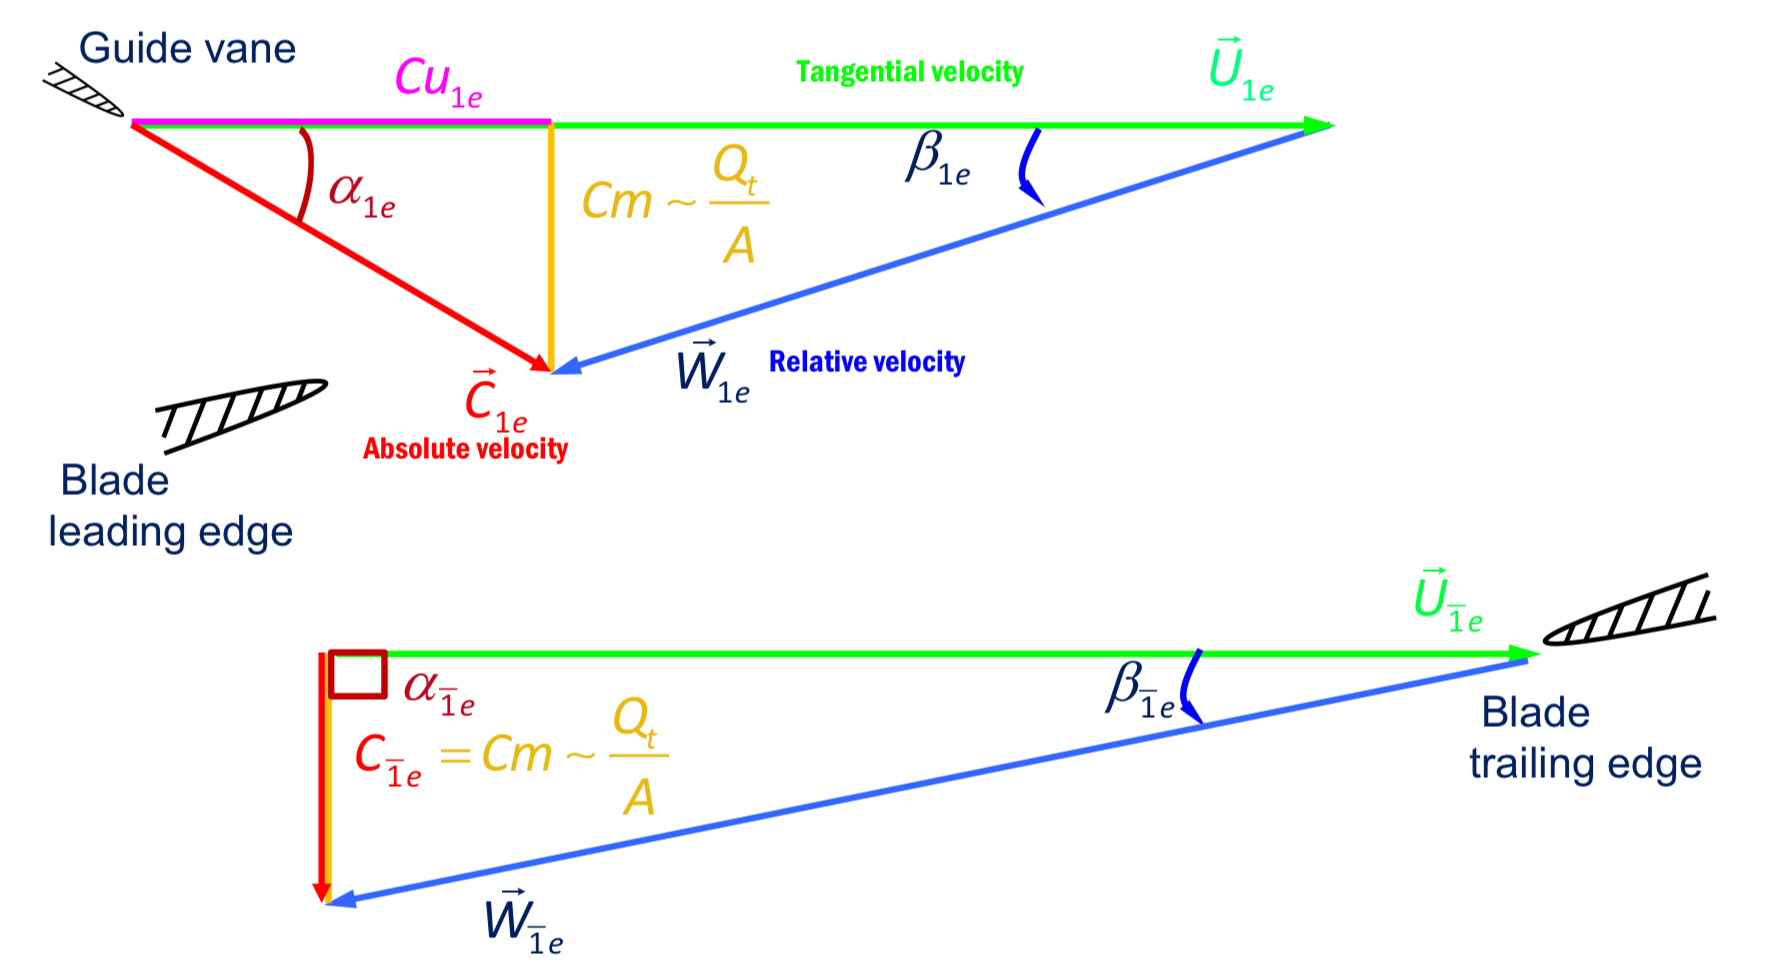
\includegraphics[width=0.7\linewidth]{IMAGES/Hydraulic/IMG_0190.jpeg}
    \caption{Maximum efficiency point}
\end{figure}

If we decrease the discharge (part load condition), then $\alpha_e$ decreases and we might get vortex rope rotating with the runner. Otherwise, $\alpha_e$ increases, we might get an axisymmetric vortex counter-rotating with respect to the runner that is cavitating.\\

\subsubsection{Deriaz turbine}
They handle mixed flow, are reversible and have adjustable runner blades.\\
A valid solution for high flexibility and high incidence of part-load.\\

\subsubsection{Kaplan runners}
Axial flow, low head.\\
Between 3-6 blades. Bulb is similar to kaplan but can handle fully axial/mixed flow and are fully submerged.\\

For the Kaplan, we aim to always have $\alpha_{\overline{1e}} = \frac{\pi}{2}$ for the BEP. We also have that $\beta_1 = \beta_{\overline{1}}$.

\subsubsection{Draft tube}
We have the following : \begin{itemize}
    \item $E_{rsc}$ : energy lost in spiral case
    \item $E_{rv}$ : energy lost in stay vanes
    \item $E_{ro}$ : energy lost in guide vanes
    \item $E_{rb}$ : energy lost in the blades
    \item $E_{rd}$ : energy lost in the draft tube
\end{itemize}

Let's denote $E_t^*$ the turbine specific energy without a draft tube and $E_t$ with a draft tube. Then $E_t - E_t^* = \frac{C_{\overline{2}}^2}{2} - \frac{C_{\overline{I}}^2}{2} + g(Z_{\overline{2}} - Z_{\overline{B}}) - E_{rd}$. With $\overline{2}$ a point at the outlet of the runner, $\overline{B}$ the surface of the water at the exit and $\overline{I}$ the outlet of the draft tube. \\
We have that $E_t - E_t^* >0$ unless $E_{rd}$ are very important.\\

\subsection{Cavitation}
It is the liquid vaporisation by pressure decrease. It happens when $p < p_{vapor}$.\\
Pressure coefficient :\begin{equation}
    Cp = \frac{p - p_{ref}}{1/2 \rho C_{ref}^2} = 1- \frac{C^2}{C_{ref}^2} + \frac{2 g L_{ref}}{C_{ref}^2}(\frac{Z_{ref} - Z}{L_{ref}}) - \frac{2g H_r}{C_{ref}^2}
\end{equation}

The cavitation onset is then : $p \leq p_v$ and $Cp \leq -\sigma = -\frac{p_{ref} - p_v}{1/2 \rho C_{ref}^2}$.\\

Let's define Froude's number : $Fr = \frac{C_{ref}}{\sqrt{2 g L_{ref}}}$ and Reynolds number : $Re = \frac{C_{ref} L_{ref}}{\nu}$. Then, we have : $Cp = 1 - \frac{C^2}{C_{ref}^2} - e_r (Re_{r,turbulence}) + \frac{1}{Fr^2} (\frac{Z_{ref}-Z}{L_{ref}}) \leq -\sigma$.\\

\subsubsection{Setting level}

The Net Positive Suction Specific Energy is defined as $NPSE = gH_{\overline{l}} - \frac{p_v}{\rho} - gZ_{ref} (J \cdot kg^{-1})$. We need a minimum setting level to avoid cavitation $h_s = Z_{ref} - Z_{\overline{B}} = Z_{\overline{1}} - Z_{\overline{B}}$, with $\overline{1}$ the exit of the turbine, $\overline{l}$ the outlet of the draft tube and $\overline{B}$ the surface of the water.\\
\begin{itemize}
    \item For turbines : $NPSE \simeq g NPSH = \frac{p_a}{\rho} - \frac{p_v}{\rho} - gh_s + \frac{C_{\overline{l}^2}}{2}$ (NPSH : Net Positive Suction Head (m))
    \item For pumps : $NPSE = \frac{p_a}{\rho} - \frac{p_v}{\rho} - gh_s = g NPSH$
    \item Thoma number : $\sigma_{th} = \frac{NPSE}{E}$
\end{itemize}
With $p_a$ the atmospheric pressure, $Z_{\overline{1}} = Z_{ref}$ and $p_v$ the saturated vapor pressure.

For pumps, cavitation happens at the inlet of the pump. \\
Main cavitation types : \begin{itemize}
    \item Suction cavitation
    \item Discharge cavitation
\end{itemize}

Main cavitation structures in pumps : \begin{itemize}
    \item Sheet cavitation at the leading edge
    \item traveling bubbles
    \item Vortical structure
\end{itemize}

\subsubsection{Cavitation damages}
\begin{itemize}
    \item Erosion 
    \item Fatigue
    \item Noise and vibrations
    \item Operation instability
    \item Performance alteration (efficiency : hub cavitation, head/discharge, runaway speed)
\end{itemize}

Cavitation wear process : \begin{itemize}
    \item Incubation process : microcraks nucleate around grain boundaries and inclusions due to elastic and plastic deformation of the surface
    \item Accumulation period : crack growth proceeds in relation to the degree of splitting, shearing and tearing action on the material
    \item SS period : the rate of crack nucleation and propagation becomes constant for the remainder of the exposure time
\end{itemize}


In axial turbine we have : \begin{itemize}
    \item Erosion risk (leading edge cavitation, tip vortex, discharge ring cavitation erosion)
    \item Efficiency alteration (hub cavitation)
\end{itemize}

In Francis turbine, we have : \begin{itemize}
    \item Efficiency alteration (traveling bubble cavitation, vortex rope)
    \item Erosion risk (leading edge cavitation)
    \item Operation instability (vortex rope, inter-blade vertices)
    \item Fatigue
\end{itemize}

Francis turbine surge : \begin{itemize}
    \item Part load resonance : pressure surge induced by the helical vortex rope 
    \item Upper part load resonance : pressure surge
    \item Full load instability : axial pulsations of the cavitation
\end{itemize}

In pumps and propellers we have : \begin{itemize}
    \item Erosion risk (impeller, pump inlet, mechanical seals, bearings)
    \item Shaft alignment
    \item Efficiency alteration
    \item Suction capability
\end{itemize}

\subsubsection{Detection techniques}

\begin{itemize}
    \item Efficiency deviation from the expected value
    \item E-monitoring (noise, vibrations)
\end{itemize}

\subsection{Hydraulic design for Francis Turbines}

Main design tools : CFD for solving the Navier Stokes equation. \\

\begin{itemize}
    \item Spiral casing : ensure even flow distribution around the runner. The runner grants a homogenous flow distribution
    \item Stay vane : mechanical function to stand the hydraulic pressure in the upstream part (thick leading edge to tolerate angle variation, thin trailing edge)
    \item Distributor : for a simple regulated turbine it is the only device to regulate the discharge/power/load. Its function is to deliver a flow angle to the runner.
    \item Runner : transform kinetic and pressure energy in mechanical energy
\end{itemize}

Each elementary turbine is defined by : \begin{itemize}
    \item 4 poles for curvature
    \item 3 abscissa + 3 thickness values
\end{itemize}

It also needs to take into account the outlet cavitation limits by changing the local curvature, blade length, number of blades, $\cdots$\\

The draft tube helps increasing the net head!\\

\quad \underline{Mechanical impacts on hydraulic design :}\\
Hydraulic profiles must be compatible with mechanical stresses. What kind of stresses ? \begin{itemize}
    \item Static head : (max when unit is stopped) casing, stay vanes, guide vanes
    \item Transient head : may affect the whole turbine
    \item Centrifugal forces : runner at runaway
    \item Fatigue phenomena
\end{itemize}

\quad \underline{Manufacturing considerations :}\\
Welded fabricated : blades are casted, a welding is needed on each side of the blade.\\
We can also have casted monobloc : one unique cast for the whole runner (small units)\\
Finally, we have forged blocks : runner machined in one or several blocks (medium runner)

\subsection{Industrial pumps}
\subsubsection{Centrifugal pumps}
Widely used to move water from one location to another. Classification : \begin{table}[hbt!]
    \centering
    \begin{tabular}{c|c}
        Flow orientation & Number of stages \\ \hline
        Radial & Single stage\\
        Mixed-flow & two stage\\
        Axial & Multistage\\
    \end{tabular}
\end{table}

Pumps for storage applications are mainly of the radial-flow type.\\
With $n_q = \frac{n \sqrt{Q}}{(\frac{H}{z_s})^{3/4}}$ and $\psi = \frac{E}{\frac{U^2}{2}}$, we have :\\

\begin{figure}[hbt!]
    \centering
    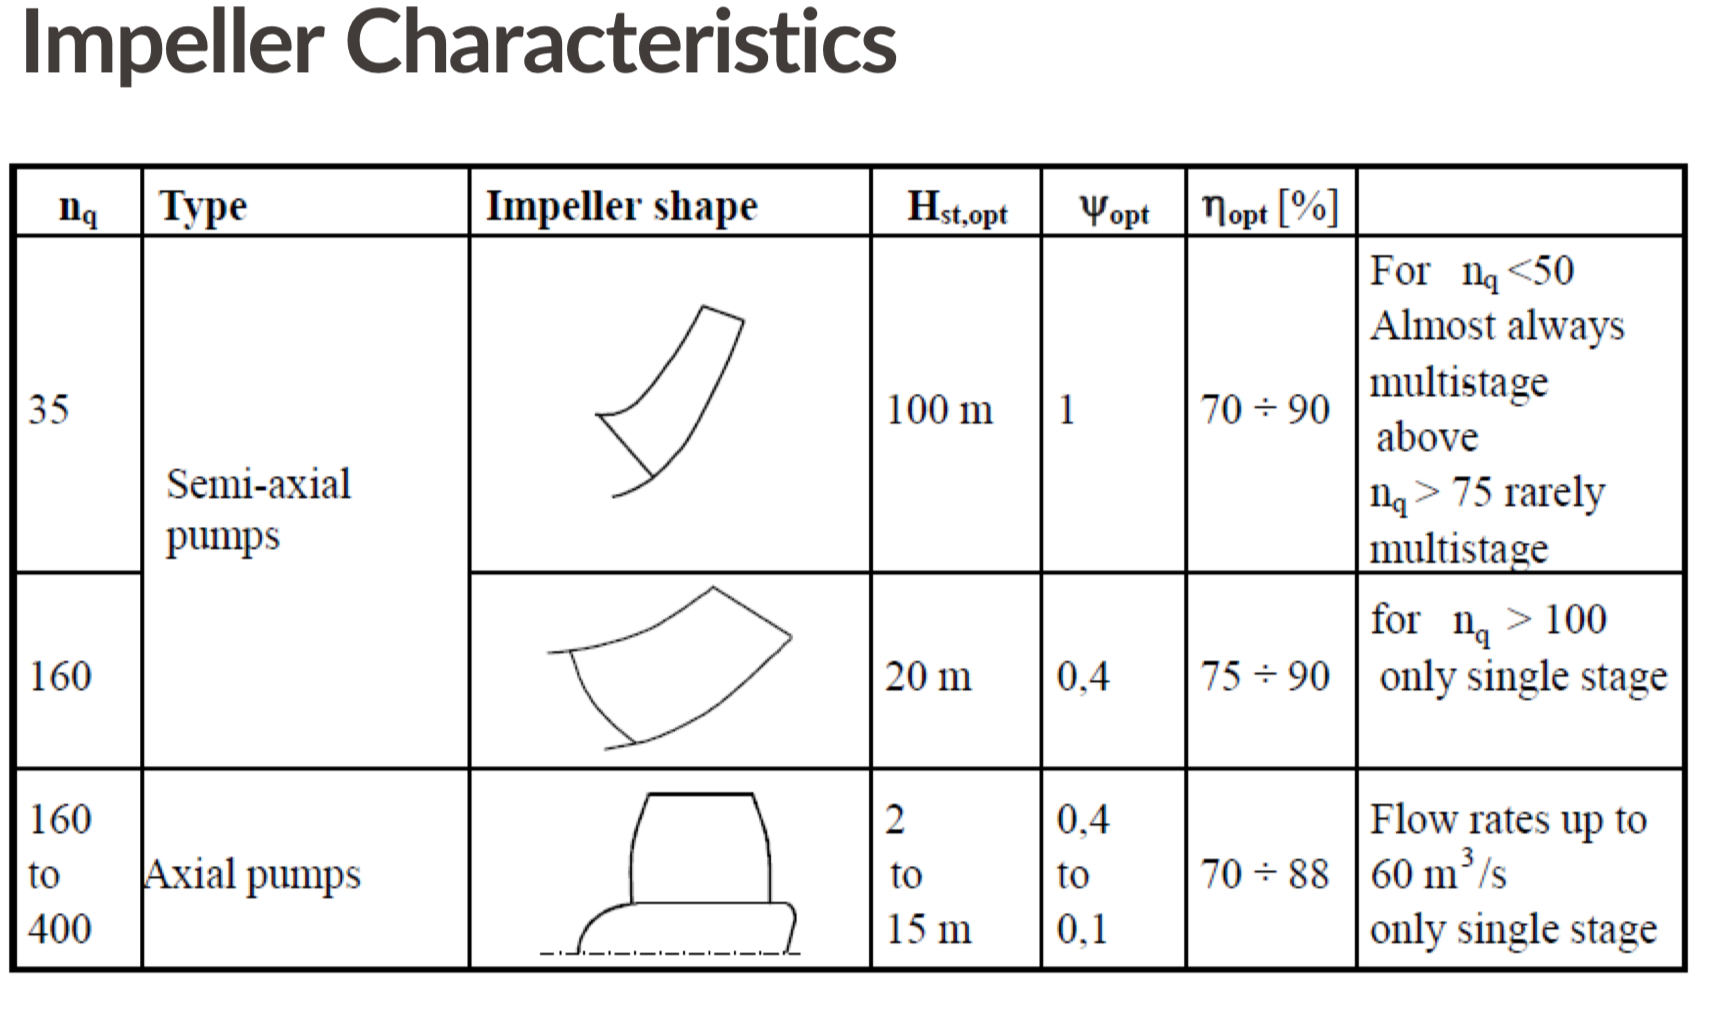
\includegraphics[width=0.8\linewidth]{IMAGES/Hydraulic/Screenshot 2024-11-21 at 10.36.50.jpeg.png}
\end{figure}

\begin{figure}[hbt!]
    \centering
    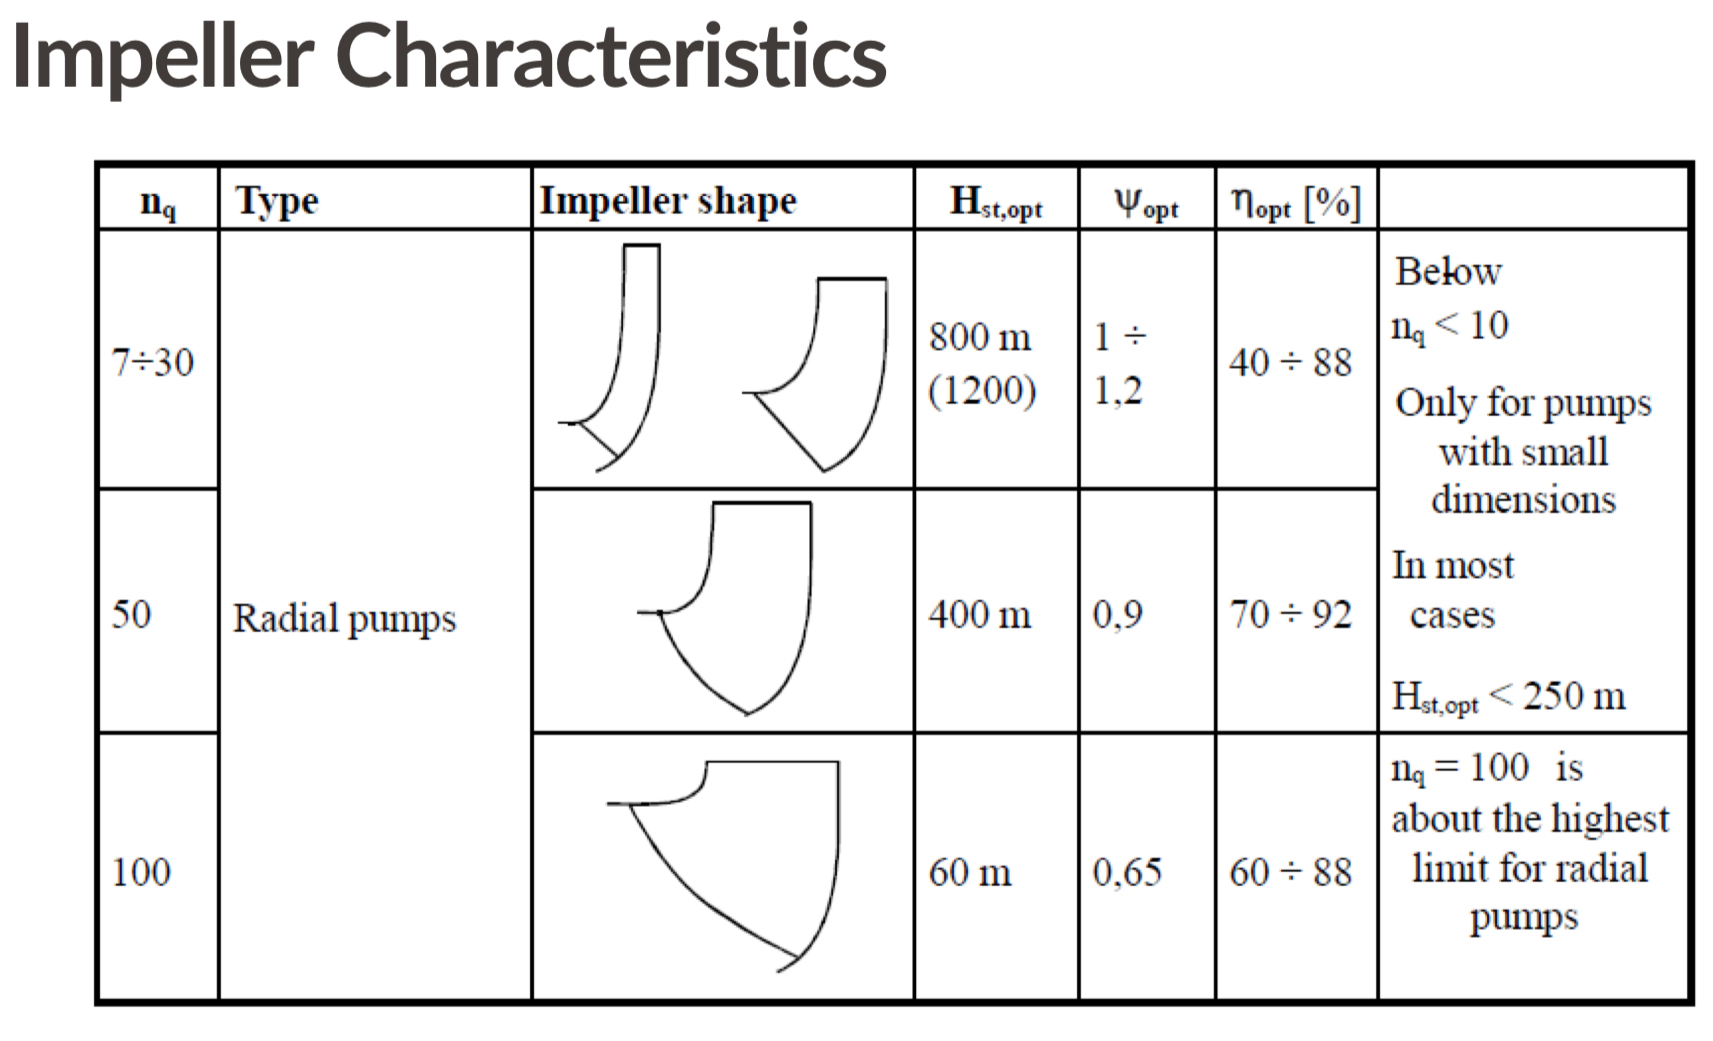
\includegraphics[width=0.8\linewidth]{IMAGES/Hydraulic/Screenshot 2024-11-21 at 10.37.29.png}
\end{figure}

Assume swirl free inlet flow : axial flow at the inlet section ($\alpha_{\overline{1e}} = \frac{\pi}{2}$) such that $E = C_{u1} U_1$.\\
At optimality, we have $P_t = P_t^{min} = \rho k_{u1e} \tan\beta_{1e} A_1 \frac{U_{1e}^3}{4}$ and $E_t = k_{u1e} \frac{U_{1e}^2}{2}$.\\
Ideally, no slip condition states that $\beta_1 = \beta_{b1}$ (angle of the blade at the outlet). In practice, $\beta_1 < \beta_{b1}$ because we have a finite number of blades and it reduces the impeller efficiency. $Cu_{1e,noslip} - Cu_{1e} = (1-\mu) U_{1e}$ with $\mu$ the slip factor/deviation angle due to : \begin{itemize}
    \item velocity differences between blade suction and pressure surface
    \item coriolis force creates a secondary flow from suction to pressure side
\end{itemize}


Losses : \begin{itemize}
    \item Leakage flow losses : part of the discharge circulates in the impeller and the side rooms. Flow rate depends on clearance, rotation in the side room, surface roughness of side room and gap. Depending on pump design leakage could be radially inward or outward for multistage pumps.
    \item Disk friction losses : drag losses due to rotation of impeller sidewalls in the fluid. Friction coefficient obtained from statistical data $P_{rm} \propto k_{rm} = f(Re)$
\end{itemize}
Pump efficiency depends on pump type, size, specific speed, liquid viscosity, rotational speed, pump execution(surface roughness).\\

Part load recirculation causes an increase in vibration, deterioration of suction performance, increase in pressure pulsation values, instabilities on the performance curve.\\
\warning Recirculation happens when the flow detaches and strong gradient perpendicular to the flow are present.\\

$NPSH_r$ (beginning of concerning cavitation) happens usually when $\frac{L_c}{D_1} = 1\%$ with $L_c$ the cavitation length.\\
$3\%$ head drop evaluation : \begin{itemize}
    \item $3\%$ head drop evaluation in closed test loops by controlled variation of suction pressure
    \item Evaluation of cavitation inception in special model pumps with optical access to impeller
    \item Predicted cavity length as a function of cavitation coefficient Cavity evolution
\end{itemize}

The suction specific speed is then : $_{ss} = \frac{n \sqrt{Q}}{(NPSH)^{3/4}}$.\\
If the pressure is too low, it is possible to add an axial inducer to pressurize the inlet section of the main pump and avoid cavitation in the main machine.\\

\quad \underline{Hydraulic forces :}\\
Axial thrust caused by the rotational and radial flow in hub and shroud side rooms which yield pressure distribution between outer and inner diameter. Resulting thrust consists of : \begin{itemize}
    \item Force on hub : $F_D = 2\pi \in p(r)rdr$
    \item Force on shroud : $F_s = 2\pi \int p(r)rdr$
    \item Impulse force due to flow redirection in impeller $F_I$
    \item Unbalanced shaft force $F_w$
\end{itemize}
Finally, we have $F_{ax} = F_D - F_s - F_I + F_w$.\\
Different approaches to balance axial thrust : \begin{itemize}
    \item Single stage pumps : balance holes, back vanes
    \item Multistage pumps : balance piston, balance disk, back-to-back impellers
\end{itemize}

Radial forces can be stationary forces due to non-uniform side room flow, pressure distribution in clearances and dynamic forces that are due to Rotor-Stator interaction and excite vibrations. 

\subsubsection{Selection of pumps}
Partial load limit (minimum discharge). Increased vibrations due to dynamic axial and radial loads. Pressure pulsations. Cavitation, motor power, thermal minimum discharge causing vaporization of liquid in the pump : $Q_{th} = \frac{P}{\rho C_p \Delta T}$.\\
Full load limit (maximum discharge). Cavitation, increased loads, motor power (radial pumps).\\

Small size standard pump : adaptation to required flow and head by trimming of impeller outer diameter.\\

Large size pump : \begin{itemize}
    \item Parameters : types of design, hydraulics set up
    \item Data requirements : flow rate, head, NPSH available, water temperature, water quality, site conditions
\end{itemize}

Hydraulic set-up : \begin{figure}[hbt!]
    \centering
    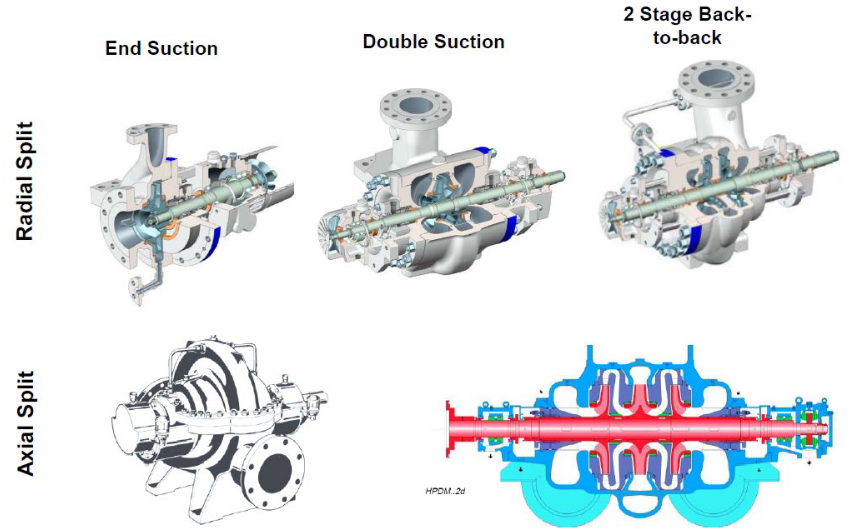
\includegraphics[width=0.5\linewidth]{IMAGES/Hydraulic/Screenshot from 2024-11-28 11-22-17.png}
\end{figure}

Interaction between pumps and the system : there are three possible configurations, serial, parallel, combined (both). The choice depends on pumped fluid, continuous and intermittent operation, pressure limit.\\
Serial configuration : best choice in case of low head application. Offers a better operating flexibility and a better efficiency. Pressure increases, discharge remains constant. \\
Parallel configuration : best choice in case of high head applications. Offers a better operating flexibility. Discharge increases and pressure increases but not as much.\\
Combined configuration : a combination of pumps in series and in parallel, with a fixed or variable drive speed, is the best choice for complex system. Offers the largest operating flexibility together with the minimum problems related to the limitation due to cavitation.\\

Pump statically stable if the pump curve has a steeper gradient as the system curve. \\
Self excited flow oscillations can occur when performance curve has positive slope, compressible element in the system. \\

\subsection{Reversible pump-turbines and pumping units}
\subsubsection{Binary group}
Two machines : electrical machine and hydraulic machine. Most common : Francis-type reversible pump-turbine. At best efficiency point : $\alpha_{\overline{e}} = \pi/2$ (if $Q<Q_0$ $\alpha$ decreases, otherwise it increases). \\
Long draft tube allow for an uniform axial flow at the inlet of the pump. Pumping mode is leading design choice in respect to the generating mode to avoid cavitation at the pump inlet section. Longer blades are needed to uniformly distribute the velocity in the blades channel.\\
The rotational speed choice can be summarized with : $n = 542.5 \frac{(H_p^*)^{0.25}}{\sqrt{Q_p^*}}$. Rotational speed in generating mode will be the same as in pumping, as the electrical machine is the same (fixed number of poles). For Francis, we have : $n = 1168.2 \frac{(H_t^*)^{0.125}}{\sqrt{Q_t^*}}$ (if used in pump-turbine do not use this relation).\\

\subsubsection{Variable speed technology}
Two solutions : full-size frequency converter, double feed asynchronous machines (cylindrical rotor with three phases winding, slip rings for excitation). Extended operating range with high performance. Allows compensating head variations and avoid cavitation.\\
Reversible pump-turbine units : 
\begin{itemize}
    \item Advantages : \begin{itemize}
        \item Fixed speed : compact, low investments costs
        \item Variable speed : efficient active power control in pumping mode, comply with large head variations, extended operating range, reactive power control
    \end{itemize}
    \item Disadvantages : \begin{itemize}
        \item Fixed speed : trade-off between pumping and generating mode, operating range restricted, long start-up time
        \item Variable speed : investment costs, specific power limited for a given rotational speed
    \end{itemize}
\end{itemize}

\subsubsection{Flow separation}
\begin{itemize}
    \item Characteristics of Rotating stall : formation of zones on adjacent channels, propagation from blade to blade at fraction of rotational speed
    \item Effect on flow : local modification of flow near walls, creation of recirculation zones causing reversing flow, impact on pressure fluctuation and vibrations
    \item Pressure fluctuation in pumping mode : larger pressure fluctuation on the vane suction side near the trailing edge
\end{itemize}

\subsubsection{Ternary group}
Three machines : electrical machine, hydraulic turbine, pump. Usually, Pelton and pump. Provides safe transient, one direction of rotation, high grade control (hydraulic by-pass), matching both pumping and generating mode (speed, length of the rotating train, required submergence). Hydraulic by-pass consists on pumping while generating. This decreases the power consumption of the plant during pumping as : $P_{tot} = P_t + P_p$.\\
\begin{itemize}
    \item Advantages : high operational flexibility, easy and short start-up time in pump mode, adjustable pump power with hydraulic by-pass, smooth transient
    \item Disadvantages : high investments costs, maintenance costs, increased ventilation losses in pumping mode (the turbine rotates)
\end{itemize}

\subsubsection{Quaternary group}
Four machines : two electrical machines and two hydraulic machines. Construction of two power houses (hydraulic turbines for generation and pump for pumping). Each group can be independently optimized, maximization of efficiency. \\
\begin{itemize}
    \item Advantages : optimization for efficiency, fastest responding pumped hydro technology
    \item Disadvantages : space requirement for 2 power houses, investments costs and maintenance
\end{itemize}

\subsection{Reduced scale physical model testing}

Similarity is defined between model (M) and prototype (P) when both have similar properties : Geometric ($\lambda_r = \frac{L_M}{L_P} = \frac{D_M}{D_P}$), Kinematic ($C_r = \frac{C_M}{C_P}$, $C$ the velocity), Dynamic ($F_r = \frac{(F_i)_M}{(F_i)_P}$, $F_i$ the force inertia, could be the viscous force or gravitational force).\\
Dimensionless numbers : Inertia force to viscosity force : $R_e = \frac{\pi n D^2}{\nu}$, $R_{ep} \simeq R_{em}$; inertia force to gravity force : $F_r = (\frac{E}{gD})^{1/2}$ \warning Most important one; Thoma number : $\sigma = \frac{NPSE}{E}$; inertia force to surface tension force : $W_e = \frac{\rho L v^2}{\sigma^*}$.\\
Head and discharge are converted into dimensionless number : \begin{itemize}
    \item $n_{ED} = \frac{nD}{E^{1/2}}$
    \item $Q_{ED} = \frac{Q}{D^2 E^{1/2}}$
    \item $P_{ED} = \frac{P_m}{\rho D^2 E^{3/2}}$
    \item $T_{ED} = \frac{T_m}{\rho D^3 E}$
\end{itemize}
One can determine the flow velocity with an electromagnetic flow meter (non-intrusive, precise). To measure the water pressure, one can use a Winter-Kennedy pressure tap. This is used to find : $Q = a \Delta p^b$ with $a_P = a_M (\frac{D_P}{D_M})^{(3-2b)} (\frac{n_P}{n_M})^{(1-2b)}$.\\
By using one transducer to get $\Delta p$ between two sections in the pipe, we have : $E = \frac{\Delta p}{\rho} + \frac{Q^2}{2} (\frac{1}{S_1^2}+\frac{1}{S_2^2})$.\\
To measure the mechanical torque, one can use a friction transducer; the axle rotates inside an oscillating part in order to prevent it from touching the fixed part. The friction torque is then $T_{fr} = FL_{fr}$ such that in turbine mode : $T_m = T + T_{fr}$ whereas in pump mode : $T_m = T-T_{fr}$.\\
For the rotational speed measurement, one can use a magnetic cell to count the number of teeth passing in front of it in a certain amount of time.\\
Errors on instruments for performance measurement should be on the order of $0.1\%$. Errors on other instrument can be higher ($5\%$ in the calibration of strain gauges). \\
Efficiency correction for \textbf{Pelton turbines :} takes into account Reynlds, Froude and Webed similitude. Often no scale-up formula are applied as on-site performance measurement are more reliable. \\
Efficiency correction for \textbf{reaction machines :} takes into account roughness of machine components, shift in energy, discharge and power factors for scale-up.\\



\end{document}